\subsection{Classification} \label{subsec:classification}

\subsubsection{Classifier}

\begin{table*}
	\caption{Overview of the classifiers used in \ac{cad} systems.}
	\small
	%\renewcommand{\arraystretch}{1.5}
	\begin{tabular}{p{.60\linewidth} p{.30\linewidth}}
		\hline \\ [-1.5ex]
		\textbf{Classifier} & \textbf{References} \\ \\ [-1.5ex]
		\hline \\ [-1.5ex]
		\textit{Rule-based method:} & $[$15,24$]$ \\ \\ [-1.5ex]
		\textit{Clustering methods:} & \\
		\quad $k$-means clustering & $[$26-28,33-34$]$ \\
		\quad \acs{knn} & $[$11,18-19$]$ \\ \\ [-1.5ex]
		\textit{Linear model classifiers:} & \\
		\quad \acs{lda} & $[$3,6,18-19,41$]$ \\
		\quad Logistic regression & $[$8-9$]$ \\ \\ [-1.5ex]
		\textit{Non-linear classifier:} & \\
		\quad \acs{qda} & $[$37$]$ \\ \\ [-1.5ex]
		\textit{Probabilistic classifier:} & \\
		\quad Naive Bayes & $[$7,17-19$]$ \\ \\ [-1.5ex]
		\textit{Ensemble learner classifiers:} & \\
		\quad AdaBoost & $[$14$]$ \\
		\quad Random forest & $[$8,31-32,35$]$ \\
		\quad Probabilistic boosting tree & $[$29-31,36$]$ \\ \\ [-1.5ex]
		\textit{Kernel method:} & \\
		\quad Gaussian processes & $[$8$]$ \\ \\ [-1.5ex]
		\textit{Sparse kernel methods:} & \\
		\quad \acs{svm} & $[$4-6,8,10-11,13-14,18-23,25,31,38-40$]$ \\
		\quad \acs{rvm} & $[$20-21$]$ \\ \\ [-1.5ex]
		\textit{Neural network:} & \\ 
		\quad Multiple layer perceptron & $[$16,22$]$ \\
		\quad Probabilistic neural network & $[$1-2,36$]$ \\ \\ [-1.5ex]
		\textit{Graphical model classifiers:} & \\
		\quad Markov random field & $[$12,21$]$ \\
		\quad Conditional random field & $[$4-5$]$ \\ \\ [-1.5ex]
		\hline
	\end{tabular}
	\label{tab:class}
\end{table*}

Once the feature vector has been extracted and eventually the complexity reduced, it is possible to make a decision and classify this feature vector to belong to \ac{cap} or healthy tissue. Classification methods used in \ac{cad} system to distinguish these two classes are summarized in Tab. \ref{tab:class}. A full review of classification methods used in pattern recognition can be found in \cite{Bishop2006}.

\setenumerate{listparindent=\parindent,itemsep=10px}
\setlist{noitemsep}
\begin{enumerate}[leftmargin=*]

\item[$-$] \textbf{\textit{Rule-based method:}}

\cite{Lv2009} make use of a decision stump classifier to distinguish \ac{cap} and healthy classes. 

\cite{Puech2009} detect \ac{cap} by implementing a given set of rules using a score medical decision making approach. The feature values are compared with a pre-defined threshold. Then, at each comparison, the final score is incremented or not, depending on the threshold and the final decision is taken depending of the final score.

\item[$-$] \textbf{\textit{Clustering methods:}} 

\acf{knn} is one of the simplest supervised machine learning classification methods. In this method, a new unlabelled vector is assigned to the most represented class from its $k$ nearest-neighbours in the feature space. The parameter $k$ is usually an odd number in order to avoid any tie case. \ac{knn} was one of the method used by \cite{Niaf2011,Niaf2012} mainly to make a comparison with different machine learning techniques. \cite{Litjens2012} used this method to roughly detect potential \ac{cap} voxels before performing a region-based classification.

$k$-means is an unsupervised clustering method in which the data have to be partitioned into $k$ clusters. The discovery of the clusters is an iterative procedure. First $k$ random centroids are defined in the feature space and each data point is assigned to the nearest centroid. Then, the centroid position for each cluster is updated by computing the mean of all the data points belonging to this particular cluster. Both assignment and updating are repeated until the centroids are stable. The number of clusters $k$ is usually defined as the number of classes. This algorithm can also be used for ``on-line'' learning. In case that new data has to be incorporated, the initial centroid positions correspond to the results of a previous $k$-means training and is followed by the assignment-updating stage previously explained.

\cite{Tiwari2007,Tiwari2009} used $k$-means in an iterative procedure. Three clusters were defined corresponding to \ac{cap}, healthy and non-prostate, respectively. $k$-means was applied iteratively and the voxels corresponding to the largest cluster were excluded under the assumption that it is assigned to ``non-prostate'' cluster. The iteration stop when the number of voxels composing all clusters remaining is smaller than a threshold.

\cite{Tiwari2008,Viswanath2008,Viswanath2008a} used $k$-means in a repetitive manner to be less sensitive to the centroids initialisation. Thus, $k$ clusters were generated $T$ times. The final assignment was performed by majority voting using a co-association matrix as proposed by \cite{Fred2005}.

\item[$-$] \textbf{\textit{Linear model classifiers:}} 

\Acf{lda} can be used as a classification method in which the optimal linear separation between two classes is found by maximizing the interclass variance and minimizing the intraclass variance (\cite{Friedman1989}). The linear discriminant function is defined as:

\begin{equation}
	\delta_{k}(\mathbf{x}_i) = \mathbf{x}_i^{\text{T}} \Sigma^{-1} \mu_k - \frac{1}{2} \mu_{k}^{\text{T}} \Sigma^{-1} \mu_k + \log (\pi_k) \ ,
	\label{eq:ldafun}
\end{equation}

\noindent where $\mathbf{x}_i$ is an unlabelled feature vector, $\Sigma$ is the covariance matrix of the training data, $\mu_k$ is the mean vector of the class $k$ and $\pi_k$ is the prior probability of class $k$.

To perform the classification, a sample $\mathbf{x}_i$ will be assigned to the class which maximizes the discriminant function:

\begin{equation}
	C(\mathbf{x}_i) = \argmax_k \delta_k(\mathbf{x}_i) \ .
	\label{eq:ldaclass}
\end{equation}
covariance matrix $\Sigma_k$ specific at each class is computed
\cite{Antic2013,Chan2003,Niaf2011,Niaf2012,Vos2012} used \ac{lda} to classify their feature vectors defining two classes \ac{cap} \textit{versus} healthy.

Logistic regression can be used to perform binary classification and can provide the probability of an observation to belong to a class. The posterior probability of one of the class $c_1$ can be written as:

\begin{equation}
	p(c_1|\mathbf{x}_i) = \frac{1}{1+\exp(-\mathbf{w}^{\text{T}}\mathbf{x}_i)} \ ,
	\label{eq:postprlr}
\end{equation}

\noindent with $p(c_2|\mathbf{x}_i) = 1 - p(c_1|\mathbf{x}_i)$ and where $\mathbf{w}$ is the vector of the regression parameters allowing to obtain a linear combination of the input feature vector $\mathbf{x}_i$.

Thus, an unlabelled observation $\mathbf{x}_i$ will be assigned to the class which maximizes the posterior probability:

\begin{equation}
	C(\mathbf{x}_i) = \argmax_k p(C=k|\mathbf{x}_i) \ .
	\label{eq:posprobreg}
\end{equation}

From Eq. \eqref{eq:postprlr}, one can see that the key to classification using logistic regression model is to infer the set of parameters $\mathbf{w}$ through a learning stage in the training set. This vector of parameters $\mathbf{w}$ can be inferred by finding the maximum likelihood estimates. This step can be performed through an optimization scheme, using a quasi-Newton method (\cite{Byrd1995}), which iteratively seeks for the local minimum in the derivative of Eq. \eqref{eq:postprlr}.

\cite{Kelm2007,Puech2009} used a logistic regression to create a linear probabilistic model in order to classify their feature vectors.

\item[$-$] \textbf{\textit{Non-linear model classifier:}} 

\cite{Viswanath2012} used the most general \acf{qda} instead of \ac{lda}. Unlike in \ac{lda} in which one assumes that the class covariance matrix $\Sigma$ is identical for all the classes, in \ac{qda}, a covariance matrix $\Sigma_k$ specific to each class is computed. Thus, Eq. \eqref{eq:ldafun} becomes:

\begin{equation}
	\delta_{k}(\mathbf{x}_i) = \mathbf{x}_i^{\text{T}} \Sigma_{k}^{-1} \mu_k - \frac{1}{2} \mu_{k}^{\text{T}} \Sigma_{k}^{-1} \mu_k + \log (\pi_k) \ .
	\label{eq:qdafun}
\end{equation}

The classification scheme in the case of the \ac{qda} is identical to Eq. \eqref{eq:ldaclass}.

\item[$-$] \textbf{\textit{Probabilistic classifier:}}

The most commonly used classifier is the naive Bayes classifier which is a probabilistic classifier assuming independence between each feature dimension (\cite{Rish2001}). This classifier is based on Bayes' theorem:

\begin{equation}
	p(C=k|\mathbf{x}) = \frac{p(C)p(\mathbf{x}|C)}{p(\mathbf{x})} \ ,
	\label{eq:bayth}
\end{equation}

\noindent where $p(C=k|\mathbf{x})$ is the posterior probability, $p(C)$ is the prior probability, $p(\mathbf{x}|C)$ is the likelihood and $p(\mathbf{x})$ is the evidence. 

However, the evidence term is usually discarded since it is not class dependent and plays the role of a normalization term. Hence, in a classification scheme, an unlabelled observation will be classified to the class which maximizes the posterior probability as:

\begin{eqnarray}
	C(\mathbf{x}_i) & = & \argmax_k p(C=k|\mathbf{x}_i) \ , \label{eq:maxbay} \\
	p(C=k|\mathbf{x}_i) & = & p(C=k) \prod_{j=1}^{n} p(x_{ij},|C=k) \ , \label{eq:postbay}
\end{eqnarray}

\noindent where $d$ is the number of dimensions of the feature vector $\mathbf{x}_i = \{x_{i1},\cdots,x_{id}\}$.

Usually, a model includes both the prior and likelihood probabilities and it is common to use an equal prior probability for each class or eventually a value depending of the relative frequency derived from the training set. Regarding the likelihood probability, it is common to choose a Normal distribution to characterize each class. Thus, each class will be characterized by two parameters: (i) the mean and (ii) the standard deviation. These parameters can be inferred from the training set by using the \ac{ml} approach.

\cite{Giannini2013,Mazzetti2011,Niaf2011,Niaf2012} used the naive Bayes classifier to classify their feature vectors to either malignant or healthy. The Normal distribution was used as the likelihood probability for that model.

\item[$-$] \textbf{\textit{Ensemble learner classifiers:}}

AdaBoost is an adaptive method based on an ensemble learner and was initially proposed by \cite{Freund1997}. AdaBoost linearly combines several weak learners resulting into a final strong classifier. A weak learner is defined as a classification method performing slightly better than random classification. Popular choices regarding the weak learner methods are: decision stump, decision tree learners (cf., \ac{id3} (\cite{Quinlan1986}), C4.5 (\cite{Quinlan1993}), \ac{cart} (\cite{Breiman1984})).

AdaBoost is considered as an adaptive method in the way that the weak learners are selected. The selection is performed in an iterative manner. At each iteration $t$, the weak learner selected $h_t$ corresponds to the one minimizing the classification error on a distribution of weights $D_t$, that is associated to the training sample. A weight $\alpha_t$ is affected at each weak learner such that:

\begin{equation}
	\alpha_t = \frac{1}{2} \ln \frac{1 - \epsilon_t}{\epsilon_t} \ ,
	\label{eq:wclssada}
\end{equation}

\noindent where $\epsilon_t$ corresponds to the classification error rate of the weak learner on the distribution of weight $D_t$.

Before performing a new iteration, the distribution of weight $D_t$ is updated such that the weight associated with the misclassified samples by $h_t$ will increase and the weights of well classified samples will decrease as shown in Eq. \eqref{eq:rewada}.

\begin{equation}
	D_{t+1}(i) = \frac{ D_t(i) \exp(-\alpha_t y_i h_{t}(\mathbf{x}_{i} ) }{ Z_t  } \ ,
	\label{eq:rewada} 
\end{equation}

\noindent where $\mathbf{x}_i$ is the $i^{\text{th}}$ sample corresponding to class $y_i$ and $Z_t$ is a normalization factor to impose that $D_{t+1}$ to be a probability distribution. 

This procedure allows to select a weak learner at the next iteration $t+1$ which will classify in priority previous misclassified samples. Thus, after $T$ iterations, the final strong classifier corresponds to the linear combination of the weak learners and the classification is performed such that:

\begin{equation}
	C(\mathbf{x}_i) = \sign \left( \sum_{t=1}^{T} \alpha_t h_t(\mathbf{x}_i) \right) \ .
	\label{eq:strclaada}
\end{equation}

\cite{Lopes2011} make use of the AdaBoost technique to perform their classification.

Random forest\footnote{Random forest implementation can be found at: \texttt{http://www.stat.berkeley.edu/\allowbreak $\sim$breiman/RandomForests/cc\_software.htm}} is a classification method which is based on creating an ensemble of decision trees and was introduced by \cite{Breiman2001}. In the learning stage, multiple decision tree learners (\cite{Breiman1984}) will be trained. However, each decision tree will be trained with a different dataset. Each of these datasets corresponds to a bootstrap sample generated by randomly choosing $n$ samples with replacement from the $N$ samples available in the original set (\cite{Efron1979}). Then, randomization is also part of the decision tree growth. At each node of the decision tree, from the bootstrap sample of $D$ dimensions, a number of $d \ll D$ dimensions will be randomly selected. Finally, the $d^{\text{th}}$ dimension splitting the best the data will be used. This best splitting is often evaluated using \ac{mi} (see Sect. \ref{subsubsec:simmea}). Finally, each tree is grown as much as possible without using any pruning procedure.

In the prediction stage, a sample is introduced in each tree and each of the tree will assign a class to this sample. Finally, it is common to use a majority voting approach to choose the final class label.

\cite{Kelm2007,Tiwari2012,Tiwari2013,Viswanath2009} make use of the random forest classifier to classify their feature vector.

\begin{figure}
\centering
	\begin{tikzpicture}
    [level distance=1.75cm,sibling distance=1.5cm,scale=.95,every node/.style={scale=0.95}, 
   edge from parent path={(\tikzparentnode) -- (\tikzchildnode)}]
	\Tree [.\node (foo) {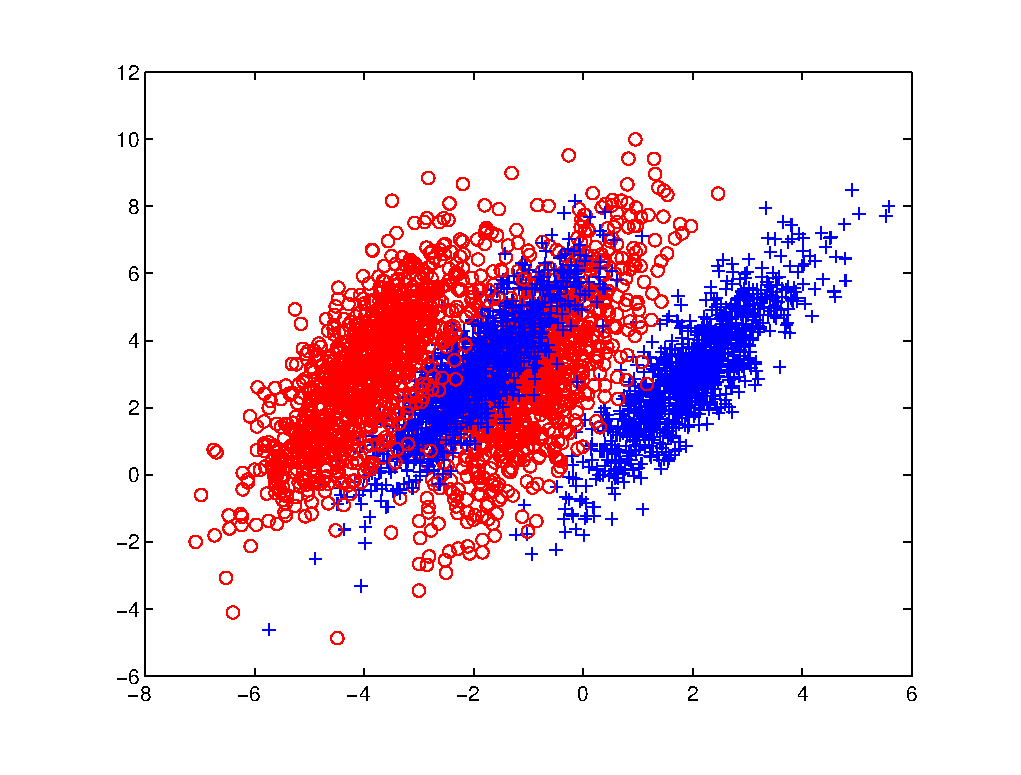
\includegraphics[width=2cm]{04_data_classification/08_classification/figures/pbt-simulation/pbt_tree_1.eps}}; 
    \edge node[auto=right] {};
    [.\node{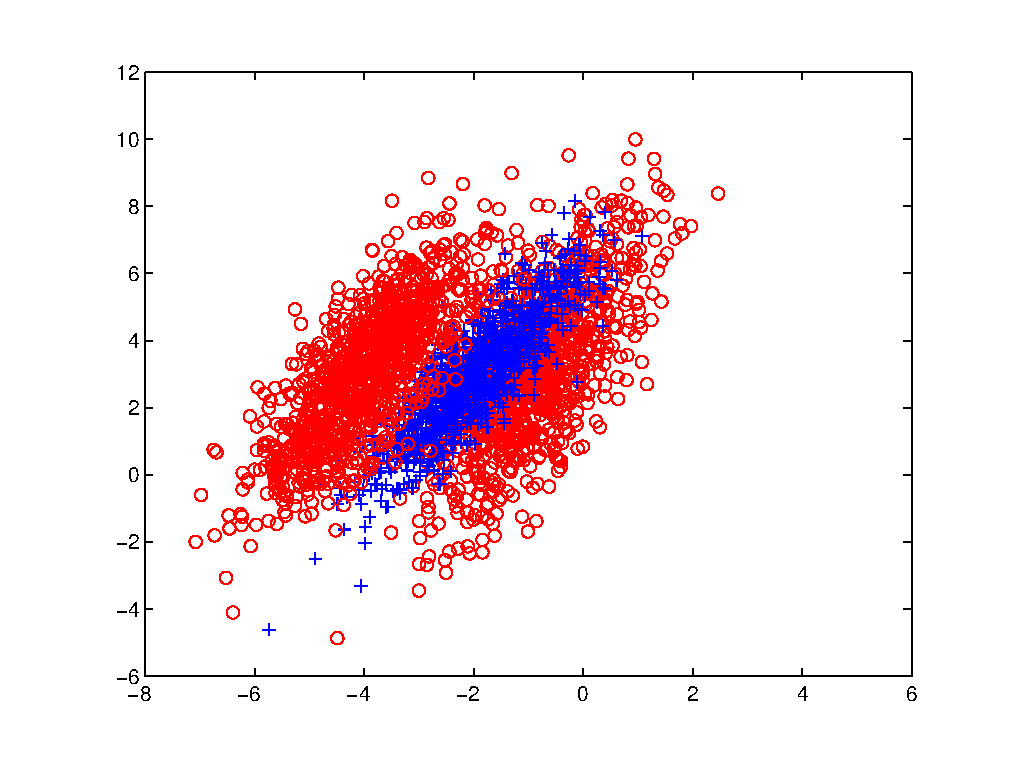
\includegraphics[width=2cm]{04_data_classification/08_classification/figures/pbt-simulation/pbt_tree_2_1.eps}};
      \edge node[auto=right] {};  
      [.\node{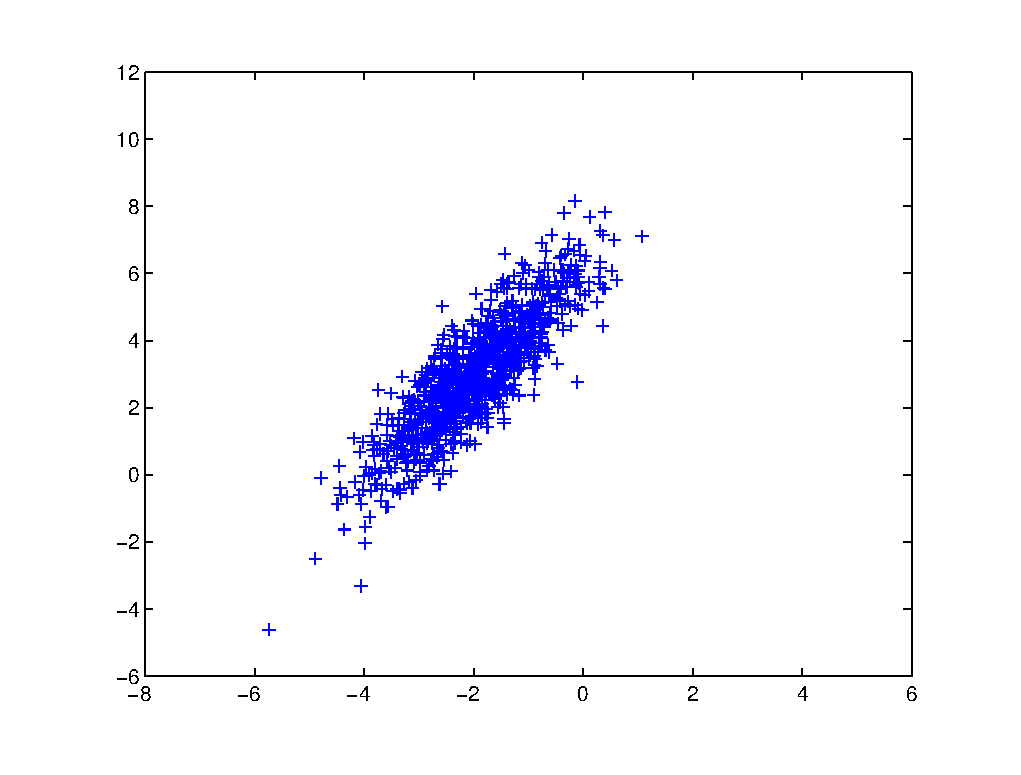
\includegraphics[width=2cm]{04_data_classification/08_classification/figures/pbt-simulation/pbt_tree_3_2.eps}}; ]
      \edge node[auto=left] {};  
      [.\node{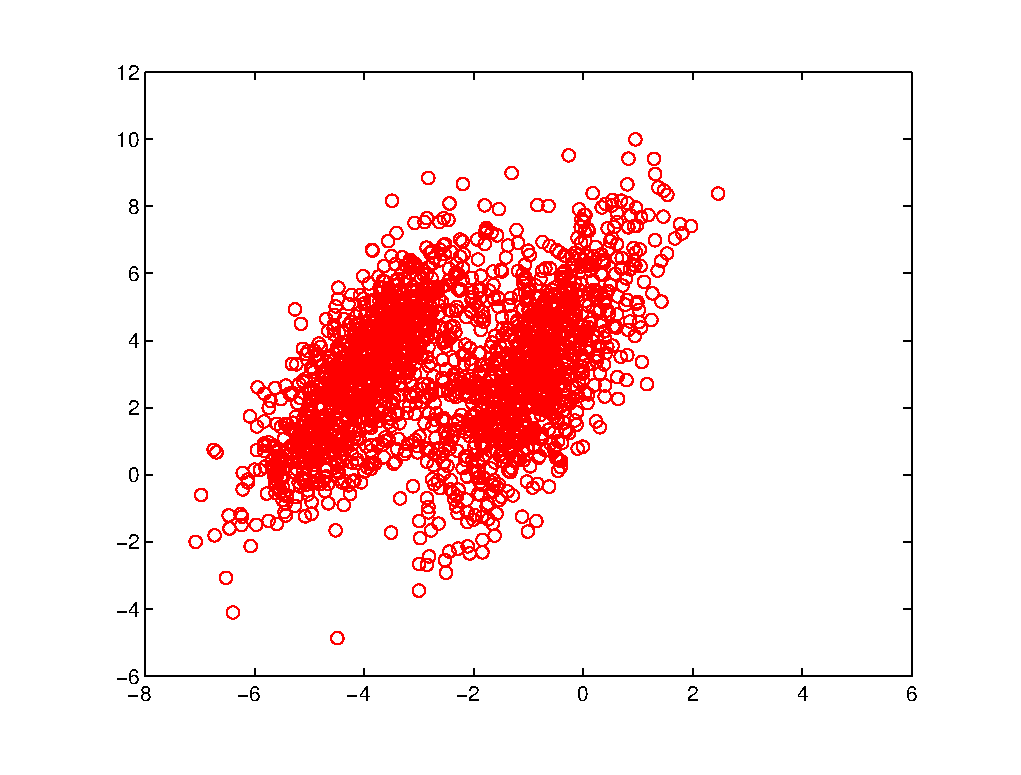
\includegraphics[width=2cm]{04_data_classification/08_classification/figures/pbt-simulation/pbt_tree_3_1.eps}}; ]
    ]
    \edge node[auto=left] {};
    [.\node{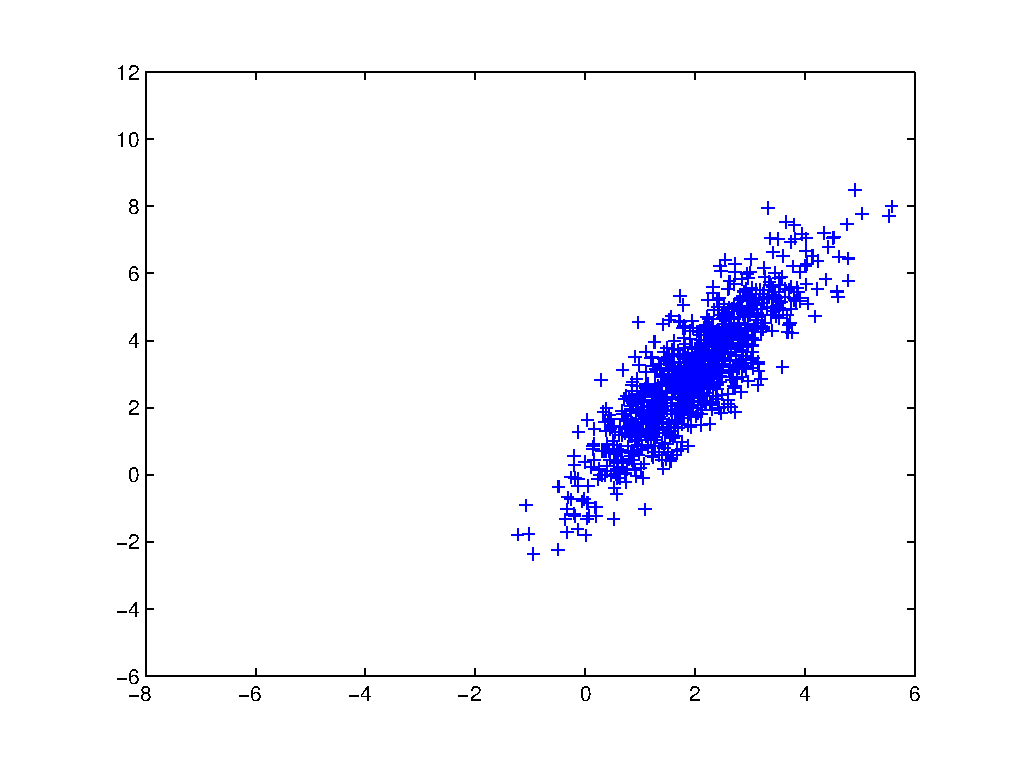
\includegraphics[width=2cm]{04_data_classification/08_classification/figures/pbt-simulation/pbt_tree_2_2.eps}};
    ]
    ];
	\end{tikzpicture}
\caption{Representation of the capabilities of the probabilistic boosting tree algorithm to split at each node of the tree the positive and negative samples.}
\label{fig:pbtsim}
\end{figure}

Probabilistic boosting-tree is an ensemble classifier method which is sharing principles from AdaBoost but using them inside a decision tree (\cite{Tu2005}). In the training stage, the probabilistic boosting-tree method grows a decision tree and at each node a strong classifier is learnt in an almost comparable scheme than AdaBoost (see Eq. \ref{eq:strclaada}). Once the strong learner is trained, the training set will be split into two subsets which will be used to train the next strong classifiers in the next descending nodes. Thus, three cases are conceivable to decide which branch to propagate each sample $\mathbf{x}_i$:

\begin{itemize}
	\item if $q(+1, \mathbf{x}_i) - \frac{1}{2} > \epsilon$ then $\mathbf{x}_i$ is propagated to the right branch set and a weight $w_i=1$ is assigned. 
	\item if $q(-1, \mathbf{x}_i) - \frac{1}{2} > \epsilon$ then $\mathbf{x}_i$ is propagated to the left branch set and a weight $w_i=1$ is assigned.
	\item else $\mathbf{x}_i$ will be propagated in both branches with $w_i=q(+1, \mathbf{x}_i)$ in the right branch and $w_i=q(-1, \mathbf{x}_i)$ in the left branch.
\end{itemize}

\noindent with $\mathbf{w} = w_i, i=\{1,\cdots,N\}$ corresponding to distribution of weights, $N$ the number of samples as in AdaBoost and $q(\cdot)$ is defined such as:

\begin{eqnarray}
	q(+1, \mathbf{x}_i) & = & \frac{\exp(2H(\mathbf{x}_i))}{1+\exp(2H(\mathbf{x}_i))} \ , \label{eq:regada1} \\
	q(-1, \mathbf{x}_i) & = & \frac{\exp(-2H(\mathbf{x}_i))}{1+\exp(-2H(\mathbf{x}_i))} \ . \label{eq:regada2}
\end{eqnarray}

Employing such a scheme tends to divide the data in such a way that positive and negative samples are naturally split as shown in Fig. \ref{fig:pbtsim}.

In the classification stage, the sample $\mathbf{x}$ is propagated through the trees, where at each node, it will be classified by the strong classifier previously learned and where an estimation of the posterior distribution will be computed. The posterior distribution will correspond to the sum of the posterior distribution at each node of the tree.

\cite{Tiwari2009a,Tiwari2012,Tiwari2010,Viswanath2011} make use of the probabilistic boosting-tree classifier.

\item[$-$] \textbf{\textit{Kernel method:}}

A Gaussian process\footnote{Gaussian process implementation can be found at: \texttt{http://www.gaussianprocess.org/gpml/\allowbreak code/matlab/doc/index.htmll}} for classification is a kernel method in which it is assumed that the data can be represented by a single sample from a multivariate Gaussian distribution (\cite{Rasmussen2005}). In the case of linear logistic regression for classification, the posterior probability can be expressed as:

\begin{eqnarray}
	p(y_i|\mathbf{x}_i,\mathbf{w}) & = & \sigma(y_i f(\mathbf{x}_i)) \ , \label{eq:gp1} \\
	f(\mathbf{x}_i) & = & \mathbf{x}_i^{\text{T}} \mathbf{w} \ , \nonumber
\end{eqnarray}

\noindent where $\sigma(\cdot)$ is the logistic function and $\mathbf{w}$ are the parameters of the model.

Thus, the classification using Gaussian processes is based on affecting a Gaussian process prior over the function $f(\mathbf{x})$ which will be characterized by a mean $\bar{f}$ and covariance functions $K$. Thus, in the training stage, the best mean and covariance functions have to be inferred in regard to our training data using a Newton optimization and a Laplacian approximation.

The prediction stage can be performed in two stages. First, for a new observation $\mathbf{x}_*$, the corresponding probability $p(f(\mathbf{x}_*)|f(\mathbf{x}))$ can be computed such that:
\begin{eqnarray}
	p(f(\mathbf{x}*)|f(\mathbf{x})) & = & \mathcal{N}( K_*K^{-1}\bar{f}, K_{**}-K_*(K')^{-1}K_*^{\text{T}} ) \ , \nonumber \\
	K' & = & K + W^{-1} \ , \label{eq:gp2} \\
	W & = & \nabla \nabla \log p(\mathbf{y}|f(\mathbf{x})) \ , \nonumber
\end{eqnarray}

\noindent where $K_{**}$ is the variance of the testing sample $\mathbf{x}_*$, $K_{*}$ is the covariance of training-testing samples $\mathbf{x}$ and $\mathbf{x}_*$.

Then, the function $f(\mathbf{x}_*)$ is squashed using the sigmoid function and the probability of the class membership can be defined such that:

\begin{equation}
	C(\mathbf{x}_*) = \sigma\left( \frac{\bar{f}(\mathbf{x_*})}{\sqrt{1+var(f(\mathbf{x}_*))}} \right) \ .
	\label{eq:gp3}
\end{equation}

Only the work of \cite{Kelm2007} used Gaussian process for classification in order to distinguish \ac{cap} in \ac{mrsi} data.

\item[$-$] \textbf{\textit{Sparse kernel methods:}}

In Gaussian process, when a prediction has to be performed, the whole training data will be used to assign a label to the new observations. That is why, this method is also called kernel method. Sparse kernel category is composed of methods which rely only on few labelled observations in order to label new observations (\cite{Bishop2006}).

\Acf{svm}\footnote{\ac{svm} implementation can be found at: \texttt{http://www.csie.ntu.edu.tw/\allowbreak $\sim$cjlin/libsvm/}} is a sparse kernel method based on finding the best linear hyperplane (non-linear separation is discussed further) which separates two classes such as the margin between the two classes is maximized (\cite{Vapnik1963}). The margin is in fact the region defined by two hyperplanes splitting the two classes, such that no points lie in between. The distance between these two hyperplanes is equal to $\frac{2}{\|\mathbf{w}\|}$ where $\mathbf{w}$ is the normal vector of the hyperplane splitting the classes. Thus, maximizing the margin is equivalent to minimizing $\|\mathbf{w}\|$. Hence, This problem is solved by an optimization approach and formalized such that:

\begin{equation}
\begin{aligned}
& \argmin_{\mathbf{w}}
& & \frac{1}{2} \| \mathbf{w}^2\| \ , \\
& \text{subject to}
& & y_i(\mathbf{w}.\mathbf{x}_i - b) \geq 1, \; i = \{ 1, \ldots, N \} \ ,
\end{aligned}
\label{eq:svm1}
\end{equation}

\noindent where $\mathbf{x}_i$ is a training sample with is corresponding class label $y_i$.

From Eq. \eqref{eq:svm1}, it is important to notice that only few points from the set of $n$ points have to be selected which will later define the hyperplane. This can be introduced in the optimization problem using Lagrange multipliers $\boldsymbol{\alpha}$. All points which are not lying on the margin will be assigned a corresponding $\alpha_i = 0$. This can be formalized as:

\begin{equation}
	\arg\min_{\mathbf{w},b } \max_{\boldsymbol{\alpha}\geq 0 } \left\{ \frac{1}{2}\|\mathbf{w}\|^2 - \sum_{i=1}^{n}{\alpha_i[y_i(\mathbf{w}\cdot \mathbf{x_i} - b)-1]} \right\} \ .
	\label{eq:svm2}
\end{equation}

The different parameters can be inferred using quadratic programming. This version of \ac{svm} is known as hard-margin since that no point can lie in the margin area. However, this is highly probable to not find any hyperplane splitting the classes such as specified previously. Thus, a soft-margin optimization approach was proposed (\cite{Cortes1995}), where points can lie into the margin but at the cost of penalty which will be minimized in the optimization process such that:

\begin{equation}
\small
\arg\min_{\mathbf{w},\mathbf{\xi}, b } \max_{\boldsymbol{\alpha},\boldsymbol{\beta} } \left\{ \frac{1}{2}\|\mathbf{w}\|^2+C \sum_{i=1}^n \xi_i - \sum_{i=1}^{n}{\alpha_i[y_i(\mathbf{w}\cdot \mathbf{x_i} - b) -1 + \xi_i]} - \sum_{i=1}^{n} \beta_i \xi_i \right\} \ .
\end{equation}

The decision to assign the label to a new observation $\mathbf{x}_i$ is taken such that:

\begin{equation}
	C(\mathbf{x}_i) = \sign \left( \sum_{n=1}^{N} \alpha_n (\mathbf{x}_n . \mathbf{x}_i) + b_0 \right) \ ,
	\label{eq:svmdec} 
\end{equation}

\noindent where $\mathbf{x}_n|n=\{1,\cdots,S\}$, $S$ being the support vectors.

\ac{svm} can also be used as a non-linear classifier by performing a kernel trick \cite{Boser1992}. The original data $\mathbf{x}$ can be projected in an high-dimensional space in which it is assumed that a linear hyperplane will split the classes. Different kernels are popular such as the \ac{rbf} kernel, polynomial kernels or Gaussian kernel.

In prostate \ac{cad} system, \ac{svm} is the most popular classification method and was used in a multitude of research works: \cite{Artan2009,Artan2010,Chan2003,Kelm2007,Litjens2011,Litjens2012,Liu2013,Lopes2011,Niaf2011,Niaf2012,Ozer2009,Ozer2010,Parfait2012,Peng2013,Sung2011,Tiwari2012,Vos2008,Vos2008a,Vos2010,Vos2012}.

\Acf{rvm} is a sparse version of Gaussian process previously presented and was proposed by \cite{Tipping2001}. \ac{rvm} is identical to a Gaussian process with following covariance function (\cite{Quinonero-Candela2002}):

\begin{equation}
	K_{RVM}(\mathbf{x}_p,\mathbf{x}_q) = \sum_{j=1}^{M} \frac{1}{\alpha_j} \Phi_j ( \mathbf{x}_p ) \Phi_j ( \mathbf{x}_q ) \ ,
 	\label{eq:rvm}
\end{equation}

\noindent where $\phi(\cdot)$ is a Gaussian basis function, $\mathbf{x}_i|i=\{1,\cdots,N\}$ are the $N$ training points and $\boldsymbol{\alpha}$ are the weights.

As mentioned in \cite{Quinonero-Candela2002}, the sparsity regarding the relevance vector arises if $j \alpha_j^{-1} = 0$. The set of parameters $\boldsymbol{\alpha}$ is inferred using the expectation maximization algorithm. \cite{Ozer2009,Ozer2010} make use of \ac{rvm} and make a comparison with \ac{svm} for the task of \ac{cap} detection.

\item[$-$] \textbf{\textit{Neural network:}} 

\begin{figure}
\centering
\def\layersep{3cm}
\begin{tikzpicture}[shorten >=1pt,draw=black!50, node distance=\layersep]
    \tikzstyle{every pin edge}=[<-,shorten <=1pt]
    \tikzstyle{neuron}=[circle,fill=black!25,minimum size=17pt,inner sep=0pt]
    \tikzstyle{input neuron}=[neuron, fill=green!20];
    \tikzstyle{output neuron}=[neuron, fill=red!80];
    \tikzstyle{hidden neuron}=[neuron, fill=blue!40];
    \tikzstyle{annot} = [text width=4em, text centered]

    % Draw the input layer nodes
    \foreach \name / \y in {1,...,3}
    % This is the same as writing \foreach \name / \y in {1/1,2/2,3/3,4/4}
        \node[input neuron] (I-\name) at (0,-\y) {\tiny $x_{ \y n }$};
        
   \node[input neuron] (I-4) at (0,-4.5) {\tiny $x_{in}$};
   \draw[dashed,draw=black!50] (I-3) -- (I-4);

    % Draw the hidden layer nodes
    \foreach \name / \y in {1,...,4}
        \path[yshift=0.5cm]
            node[hidden neuron] (H-\name) at (\layersep,-\y cm) {\tiny $h_{ \y }\left(\sum \cdot \right)$};
            
    \node[hidden neuron] (H-5) at (\layersep,-5.5 cm) {\tiny $h_{j}\left(\sum \cdot \right)$};
    \draw[dashed,draw=black!50] (H-4) -- (H-5);

    % Draw the output layer node
    	\node[output neuron,pin={[pin edge={->}]right:$C_{0}$}, right of=H-2] (O-1) {\tiny $\sigma\left(\sum \cdot \right)$};
    	\node[output neuron,pin={[pin edge={->}]right:$C_{1}$}, right of=H-4] (O-2) {\tiny $\sigma\left(\sum \cdot \right)$};

    % Connect every node in the input layer with every node in the
    % hidden layer.
    \foreach \source in {1,...,4}
        \foreach \dest in {1,...,5}
        		\draw[shorten >=1pt,->,draw=black!50] (I-\source)  -- (H-\dest);
            %\path (I-\source) edge (H-\dest);
    
    % Draw the annotation for the weight for the first and last connections       
    \draw[shorten >=1pt,->,draw=black!50] (I-1) -- (H-1) node [midway, above] (w111) {\scriptsize $w_{11}^{(1)}$};
    \draw[shorten >=1pt,->,draw=black!50] (I-4) -- (H-5) node [midway, below] (w145) {\scriptsize $w_{ij}^{(1)}$};

    % Connect every node in the hidden layer with the output layer
    \foreach \source in {1,...,5}
    		\foreach \dest in {1,...,2}
        		\draw[shorten >=1pt,->,draw=black!50] (H-\source)  -- (O-\dest);
        %\path (H-\source) edge (O);
        
    % Draw the annotation for the weight for the first and last connections       
    \draw[shorten >=1pt,->,draw=black!50] (H-1) -- (O-1) node [midway, above] (w211) {\scriptsize $w_{11}^{(2)}$};
    \draw[shorten >=1pt,->,draw=black!50] (H-5) -- (O-2) node [midway, below] (w251) {\scriptsize $w_{kj}^{(2)}$};

    % Annotate the layers
    \node[annot,above of=H-1, node distance=1cm] (hl) {\footnotesize Hidden layer};
    \node[annot,left of=hl] {\footnotesize Input layer};
    \node[annot,right of=hl] {\footnotesize Output layer};
\end{tikzpicture}
\caption{Representation of a neural network of the multilayer perceptron family.}
\label{fig:mlp}
\end{figure}

Multilayer perceptron is a feed-forward neural network considered as well as the most successful model of this kind in pattern recognition (\cite{Bishop2006}). The most well spread model used is based on a two layers model where a prediction of an observation is computed as:

\begin{equation}
	C(\mathbf{x}_n,w_{ij}^{(1)},w_{kj}^{(2)}) = \sigma \left[ \sum_{j=0}^{M} w_{kj}^{(2)} \  h \left( \sum_{i=0}^{D} w_{ij}^{(1)} x_{in} \right) \right] \ ,
	\label{eq:annmlp}
\end{equation}

\noindent where $h(\cdot)$ and $\sigma(\cdot)$ are two activation functions usually non-linear, $w_{ij}^{(1)}$ and $ w_{kj}^{(2)}$ are the weights associated with the linear combination with the input feature $\mathbf{x}_n$ and the hidden unit, respectively.

A graphical representation of this network is presented in Fig. \ref{fig:mlp}. Relating Fig. \ref{fig:mlp} with Eq. \eqref{eq:annmlp}, it can be noted that this network is composed of some successive non-linear mapping of the input data. First, a linear combination of the input vector $\mathbf{x}_i$ is performed into some hidden units through a set of weights $w_{ij}^{(1)}$. This combination becomes non-linear by the use of the activation function $h(\cdot)$ which is usually chosen to be a sigmoid function. Then, a linear combination of these hidden units is performed into the output of the neural network through a set of weights $w_{kj}^{(2)}$. This combination is also mapped non-linearly using an activation function $\sigma(\cdot)$ which is usually a logistic function.

Thus, the training of such a network resides in finding the best weights $w_{ij}^{(1)}$ and $ w_{kj}^{(2)}$ which will model our data the best. The error of this model can be computed such that:

\begin{equation}
	E(w_{ij}^{(1)},w_{kj}^{(2)}) = \frac{1}{2} \sum_{n=1}^{N} \left( C(\mathbf{x}_n,w_{ij}^{(1)},w_{kj}^{(2)}) - y(\mathbf{x}_n) \right) ^{2} \ ,
	\label{eq:mlpcost}
\end{equation}

\noindent where $\mathbf{x}_n|n=\{1,\cdots,N\}$ are the $N$ training vectors with their corresponding class label $y(\mathbf{x}_n)$.

Thus the best set of weights can be inferred in an optimization framework such that:

\begin{equation}
	\argmin_{w_{ij}^{(1)},w_{kj}^{(2)}} E(w_{ij}^{(1)},w_{kj}^{(2)}) \ . 
	\label{eq:mlpopt}
\end{equation}

This optimization can be performed using a gradient descent method where the derivative of Eq. \eqref{eq:mlpcost} can be computed using the backpropagation algorithm proposed by \cite{Rumelhart1988}.

\cite{Matulewicz2013,Parfait2012} used this method to classify \ac{mrsi} spectra.

\begin{figure}
\centering
\def\layersep{3cm}
\def\finallayersep{2.2cm}
\begin{tikzpicture}[shorten >=1pt,draw=black!50, node distance=\layersep]
    \tikzstyle{every pin edge}=[<-,shorten <=1pt]
    \tikzstyle{neuron}=[circle,fill=black!25,minimum size=20pt,inner sep=0pt]
    \tikzstyle{input neuron}=[neuron, fill=green!20];
    \tikzstyle{output neuron}=[neuron, fill=red!80];
    \tikzstyle{hidden neuron}=[neuron, fill=blue!20];
    \tikzstyle{summation neuron}=[neuron, fill=blue!40];
    \tikzstyle{annot} = [text width=4em, text centered]

    % Draw the input layer nodes
    \foreach \name / \y in {1,...,3}
    % This is the same as writing \foreach \name / \y in {1/1,2/2,3/3,4/4}
        \node[input neuron] (I-\name) at (0,-\y-1) {\tiny $x_{ \y n }$};
        
   \node[input neuron] (I-4) at (0,-5.5) {\tiny $x_{in}$};
   \draw[dashed,draw=black!50] (I-3) -- (I-4);
   
   % Draw the pattern layer
   \node[hidden neuron] (H-1) at (\layersep,0 cm) {\tiny $h_{11}\left( \cdot \right)$};
   \node[hidden neuron] (H-2) at (\layersep,-1 cm) {\tiny $h_{21}\left( \cdot \right)$};
   \node[hidden neuron] (H-3) at (\layersep,-2.5 cm) {\tiny $h_{31}\left( \cdot \right)$};
   \draw[dashed,draw=black!50] (H-2) -- (H-3);
   
   \begin{pgfonlayer}{background}
	\path (H-1.west |- H-1.north)+(-0.2,0.2) node (a) {};
    \path (H-3.east |- H-3.south)+(+0.2,-0.2) node (b) {};
          
    \path[fill=blue!10,rounded corners, draw=blue!50, dashed] (a) rectangle (b);
   \end{pgfonlayer}
   
   \node[hidden neuron] (H-4) at (\layersep,-4.5 cm) {\tiny $h_{12}\left( \cdot \right)$};
   \node[hidden neuron] (H-5) at (\layersep,-5.5 cm) {\tiny $h_{22}\left( \cdot \right)$};
   \node[hidden neuron] (H-6) at (\layersep,-7 cm) {\tiny $h_{32}\left( \cdot \right)$};
   \draw[dashed,draw=black!50] (H-5) -- (H-6);
   
   \begin{pgfonlayer}{background}
	\path (H-4.west |- H-4.north)+(-0.2,0.2) node (c) {};
    \path (H-6.east |- H-6.south)+(+0.2,-0.2) node (d) {};
          
    \path[fill=blue!10,rounded corners, draw=blue!50, dashed] (c) rectangle (d);
   \end{pgfonlayer}
   
   % Draw the summation layer
   \begin{scope}[node distance=2cm]
   \node[summation neuron, right of=H-2] (S-1) {\tiny $\sum_1 \cdot $};
   \node[summation neuron, right of=H-5] (S-2) {\tiny $\sum_2 \cdot $};
   \end{scope}
   
   % Draw the decision layer
   \node[output neuron,pin={[pin edge={->}]right:$C$},] at (3*\finallayersep,-3.5 cm) (O) {$\sigma \left( \cdot \right)$};
   
   % Draw the networking from input layer to pattern layer
   \foreach \source in {1,...,4}
   		\foreach \dest in {1,...,6}
   				\draw[shorten >=1pt,->,draw=black!50] (I-\source)  -- (H-\dest);
   				
   % Draw the networking from pattern layer to summation layer
   \foreach \source in {1,...,3}
   		\draw[shorten >=1pt,->,draw=black!50] (H-\source)  -- (S-1);
   		
   	\foreach \source in {4,...,6}
   		\draw[shorten >=1pt,->,draw=black!50] (H-\source)  -- (S-2);
   		
   	% Draw from summation layer to ouput
   	\draw[shorten >=1pt,->,draw=black!50] (S-1)  -- (O);
   	\draw[shorten >=1pt,->,draw=black!50] (S-2)  -- (O);
  
    % Annotate the layers
    \node[annot,above of=H-1, node distance=1cm] (hl) {\footnotesize Pattern layer};
    \node[annot,left of=hl] {\footnotesize Input layer};
    \begin{scope}[node distance=2cm]
    \node[annot,right of=hl] {\footnotesize Summation layer};
    \end{scope}
    \node[annot,above of=O, node distance=4.5cm] (o) {\footnotesize Decision layer};
\end{tikzpicture}
\caption{Representation of a neural network of the probabilistic neural network family.}
\label{fig:pnn}
\end{figure}

Probabilistic neural networks are another type of feed-forward networks which can be derived from the multilayer perceptron case and was proposed by \cite{Specht1988}. This classifier can be modelled by changing the activation function $h(\cdot)$ in Eq. \eqref{eq:annmlp} to an exponential function such that:

\begin{equation}
	h(\mathbf{x}_n) = \exp \left( - \frac{ (\mathbf{w}_j - \mathbf{x})^{\text{T}}(\mathbf{w}_j - \mathbf{x}) }{2\sigma^2} \right) \ ,
	\label{eq:pnn1}
\end{equation}

\noindent where $\sigma$ is a free parameter.

The other difference of the probabilistic neural network with the multilayer perceptron resides in the architecture as shown in Fig. \ref{fig:pnn}. This network is formed by two hidden layers. The first hidden layer corresponds to the pattern layer which is the mapping done using Eq. \eqref{eq:pnn1}. This pattern layer is sub-divided into groups corresponding to the class. The second hidden layer corresponds to the summation layer which simply sums the output of each sub-group of the pattern layer. This method was used  by \cite{Ampeliotis2007,Ampeliotis2008,Viswanath2011} in order to perform the classification of their feature vector.

\item[$-$] \textbf{\textit{Graphical model classifiers:}}

Markov random fields can also be used as a lesion segmentation method to detect \ac{cap}. First, we can define $s$ as a pixel which will belong to a certain class denoted by $\omega_s$. The labelling process can be noted as $\omega = \{\omega_s, s \in I\}$ where $I$ is the set of all the pixels inside the image. The observations corresponding to \ac{si} in the image are noted $\mathcal{F} = \{ f_s | s \in I \}$. Thus, the image process $\mathcal{F}$ represents the deviation from the labelling process $\omega$ (\cite{Kato2001}). Hence, lesion segmentation is equivalent to estimate to estimating the best $\hat{\omega}$ which maximizes the posterior probability $p(\omega|\mathcal{F})$. Thus, using a Bayesian approach, this can be formulated such that:

\begin{equation}
	p(\omega|\mathcal{F}) = \argmax_{\omega} \prod_{s \in I} p(f_s | \omega_s) p(\omega) \ .
	\label{eq:mrf1}
\end{equation}

It is generally assumed that $p(f_s | \omega_s)$ follows a Gaussian distribution and that the pixels classes $\lambda = \{1,2\}$ for a binary classification will be characterized by their respective mean $\mu_{\lambda}$ and standard deviation $\sigma_{\lambda}$. Then, $\omega$ is supposed to be a Markov random field thus:

\begin{equation}
	p(\omega) =  \frac{1}{Z} \exp\left( -U(\omega) \right)  \ ,
	\label{eq:mrf2}
\end{equation}

\noindent where $Z$ is a normalization factor to obtain a probability value, $U(\cdot)$ is the energy function.

Thus the segmentation problem can be solved as an optimization problem where the energy function $U(\cdot)$ has to be minimized. There are different possibilities to define the energy function $U(\cdot)$. However, this is common to define the energy function such that it combines two type of potential function: (i) a local term relative to the pixel itself and (ii) a smoothing prior which embeds neighbourhood information which will more or less penalizes the energy function to obtain more or less homogeneous region. This optimization of such function can be performed with an algorithm such as iterated conditional modes (\cite{Kato2001}).

\cite{Liu2009,Ozer2010} used Markov random fields as an unsupervised method to segment lesions in multi-parametric \ac{mri} images.

\cite{Artan2009,Artan2010} used conditional random fields instead of Markov random fields to segment their \ac{mri} images. The difference between these two methods reside in the fact that conditional probabilities are used such as:

\begin{equation}
	p(\omega|\mathcal{F}) =  \frac{1}{Z} \exp \left[ - \sum_{s \in I} V_{C1}(\omega_s|\mathcal{F}) - \sum_{\{s,r\} \in C } V_{C2} (\omega_s,\omega_r|\mathcal{F})  \right] \ .
\label{eq:crf}
\end{equation}

\noindent $V_{C1}(\cdot)$ is the state (or partition) feature function and $V_{C2}(\cdot)$ is the transition (or edge) feature function (\cite{Kato2012}).

\end{enumerate}

\subsubsection{Model validation}

\begin{table}
	\caption{Overview of the model validation techniques used in \ac{cad} systems.}
	\small
	%\renewcommand{\arraystretch}{1.5}
	\begin{tabular}{p{.55\linewidth} p{.35\linewidth}}
		\hline \\ [-1.5ex]
		\textbf{Model validation techniques} & \textbf{References} \\ \\ [-1.5ex]
		\hline \\ [-1.5ex]
		\quad \acs{loo} & $[$1-8,11,17-21,23,25,32,36,38-40$]$ \\ \\ [-1.5ex]
		\quad \acs{kcv} & $[$10,22,28-32,37,35,41$]$ \\ \\ [-1.5ex]
		\hline
	\end{tabular}
	\label{tab:valmod}
\end{table}

In pattern recognition, the use of model validation techniques to assess the performance of trained classifiers is quite important. Two techniques are broadly used in the development of \ac{cad} system and are summarized in Tab. \ref{tab:valmod}.

The most popular technique used in \ac{cad} systems (see Tab. \ref{tab:valmod}) is the \acf{loo} technique. From the whole data, one patient is kept to validate and the other cases are used to train. This manipulation is repeated until each patient is used for validation. This technique is popular when working with medical data due to the restricted number of patients included in datasets. Thus, it allows to train on a fair number of patients even with a small dataset. However, this technique suffer from high variance and can considered as a non reliable estimate (\cite{Efron1983}).

The other very well known technique used for assessing classifier is the \acf{kcv} technique. This technique is based on splitting the dataset into $k$ subsets where the samples are randomly selected. Then, one fold is kept for the validation and the remaining subsets for training. The classification is then repeated as in the \ac{loo} technique. In our review, the typical values used for $k$ were set to three and five. This technique is more appropriate than the previous one since that it does not suffer from large variance. However, the number of patients in the dataset needs to be large enough to apply such technique.

\subsubsection{Evaluation measure}\label{subsubsec:eval}

\begin{table}
	\caption{Overview of the evaluation metrics used in \ac{cad} systems.}
	\small
	%\renewcommand{\arraystretch}{1.5}
	\begin{tabular}{p{.55\linewidth} p{.35\linewidth}}
		\hline \\ [-1.5ex]
		\textbf{Evaluation metrics} & \textbf{References} \\ \\ [-1.5ex]
		\hline \\ [-1.5ex]
		\quad Accuracy & $[$4-5,12,25,31$]$ \\ \\ [-1.5ex]
		\quad Sensitivity - Specificity & $[$4-5,7,12,14,17,20-23,25,27-28,33-34$]$ \\ \\ [-1.5ex]
		\quad \acs{roc} - \acs{auc} & $[$2-3,6-9,13-19,23,29-32,35-40$]$ \\ \\ [-1.5ex]
		\quad \acs{froc} & $[$10-11,41$]$ \\ \\ [-1.5ex]
		\quad Dice's coefficient & $[$4-5,12,20$]$ \\ \\ [-1.5ex]
		\hline
	\end{tabular}
	\label{tab:evatec}
\end{table}

Several metrics can be used in order to assess the performance of the classifier trained when tested on the test data. The techniques used for evaluation of the \ac{cad} system for \ac{cap} detection are summarized in Tab. \ref{tab:evatec}.

Using the classification approach previously presented, each voxel in the \ac{mri} image will be classified into a class. Comparison with a ground-truth can give rise to a confusion matrix by counting true positive, true negative, false positive and false negative samples. From this analysis, different statistics can be extracted. 

The first statistic used is the accuracy which computes the ratio of true detection over the number of samples. However, depending on the strategy employed in the \ac{cad} work-flow, this statistic can be highly biased by a high number of true negative samples which will boost the accuracy score and does not represent the actual performance of the classifier.

That is why, the most common statistic computed are sensitivity and specificity which are giving a full overview of the performance of the classifier trained. Sensitivity is also called the true positive rate and is equal to the ratio of the true positive samples over the true positive added with the false negative samples. Specificity is also named the true negative rate and is equal to the ratio of the true negative samples over the true negative added with the false positive samples.

These both statistics gave rise to the \acf{roc} analysis. This analysis represents graphically the sensitivity as a function of (1 - specificity), which is in fact the false positive rate, by varying the discriminative threshold of the classifier. By varying this threshold, more true negative samples will be found but at the cost to detect also more false negative. However, this fact is interesting in \ac{cad} since that it could be possible to obtain a high sensitivity and to ensure that no cancers were missed even if more false alarm will have to be investigated. A statistic derive from \ac{roc} analysis is the \acf{auc} which corresponds to the area under the \ac{roc} and is a measure used to make comparison between models. 

The previous method could have been classified on pixel-based evaluation method. However, a cancer can be also considered as a region. \Acf{froc} extends the \ac{roc} analysis but at region-based level. The same confusion matrix can be computed were the sample are not pixels any more but refer to a lesion. However, this is important to define what is a true positive sample in that case. Usually, a lesion is considered as a true positive sample if the region detected by the classifier and the one inside the ground-truth are overlapping ``enough''. ``Enough'' is defined by each researcher and can correspond to one pixel only!!!

Finally, Dice's coefficient is sometimes computed which is corresponding to the similarity of a lesion between the ground-truth and the output of the classifier. This coefficient corresponds to the ratio of twice the number of pixels in common over the sum of the pixels of the lesions in the ground-truth and the output of the classifier.